% \documentclass[handout]{beamer}
\documentclass{beamer}

\mode<presentation>
{
  \usetheme{default}
  \usefonttheme[onlymath]{serif}
  % \usetheme{Singapore}
  % \usetheme{Warsaw}
  % \usetheme{Malmoe}
  % \useinnertheme{circles}
  % \useoutertheme{infolines}
  % \useinnertheme{rounded}

  \setbeamercovered{transparent=5}
}

\usepackage[english]{babel}
\usepackage[latin1]{inputenc}
\usepackage{textpos,alltt,listings,multirow,ulem,siunitx}
\newcommand\hmmax{0}
\newcommand\bmmax{0}
\usepackage{bm}

% font definitions, try \usepackage{ae} instead of the following
% three lines if you don't like this look
\usepackage{mathptmx}
\usepackage[scaled=.90]{helvet}
% \usepackage{courier}
\usepackage[T1]{fontenc}
\usepackage{tikz}
\usetikzlibrary[shapes,shapes.arrows,arrows,shapes.misc,fit,positioning]

% \usepackage{pgfpages}
% \pgfpagesuselayout{4 on 1}[a4paper,landscape,border shrink=5mm]

\usepackage{JedMacros}

\title{Computational methods for ice flow simulation \\
with applications to Jakobshavn Isbr{\ae}}
\subtitle{Diss. ETH No. 19948}

\author{Jed Brown}


% - Use the \inst command only if there are several affiliations.
% - Keep it simple, no one is interested in your street address.
\institute
{VAW, ETH Z\"urich}

\date{2011-09-06}

% This is only inserted into the PDF information catalog. Can be left
% out.
\subject{Talks}


% If you have a file called "university-logo-filename.xxx", where xxx
% is a graphic format that can be processed by latex or pdflatex,
% resp., then you can add a logo as follows:

% \pgfdeclareimage[height=0.5cm]{university-logo}{university-logo-filename}
% \logo{\pgfuseimage{university-logo}}



% Delete this, if you do not want the table of contents to pop up at
% the beginning of each subsection:
% \AtBeginSubsection[]
% {
% \begin{frame}<beamer>
%   \frametitle{Outline}
%   \tableofcontents[currentsection,currentsubsection]
% \end{frame}
% }

\AtBeginSection[]
{
  \begin{frame}<beamer>
    \frametitle{Outline}
    \tableofcontents[currentsection]
  \end{frame}
}

% If you wish to uncover everything in a step-wise fashion, uncomment
% the following command:

% \beamerdefaultoverlayspecification{<+->}

\begin{document}
\lstset{language=C}
\normalem

\begin{frame}
  \titlepage
\end{frame}

\section{Perspective}
\begin{frame}{Grand Challenge Problems}
  \begin{block}{Global Prosperity Optimization}
    Maximize the prosperity functional by adjusting energy policy, urban and groundwater planning, geoengineering projects, etc.
  \end{block}
  \begin{block}{Ice Sheet Stability Questions (short-term connection via Ocean)}
    \begin{itemize}
    \item Where is the stability manifold at Pine Island, Thwaites, and other outlet glaciers relative to current trajectories?
    \item In the event of entering an unstable regime, how rapid would the resulting sea level rise be?
    \item What possible anthropogenic sources have the most influence on stability and related sea level rise?
    \item What are the errors associated with these computations?
    \item Which field work and remote sensing studies would provide the most cost-effect way to reduce uncertainty?
    \end{itemize}
  \end{block}
\end{frame}

\begin{frame}{Where does computation fit in?}
  \begin{itemize}
  \item Scientific applications: use computation to investigate scientific questions
    \begin{itemize}
    \item non-model problems: messy, coupled, highly nonlinear
    \item do not want to spend career focusing on methods
    \item slow to respond to developments in mathematics
    \item difficult to evaluate performance/robustness without implementing
    \end{itemize}
  \item Applied mathematics: create and analyze new methods
    \begin{itemize}
    \item identify key ingredients needed for robustness and accuracy
    \item well-posed formulations and (quadratically) convergent methods to provide quantitative answers to scientific questions (``why'', ``how'')
    \item demonstrate on simplified models (geometry, boundary conditions, materials)
    \item efficient implementation not important: focus on asymptotics
    \end{itemize}
  \item Scientific software: make methods available and performant
    \begin{itemize}
    \item modify methods for robustness on wider variety of problems
    \item make interfaces usable by non-experts
    \item decouple from problem specification
    \item implementation efficiency is important, follow new hardware
    \item solved problems should not need to be revisited
    \item reusable components: experiment in minutes instead of months
    \end{itemize}
  \end{itemize}
\end{frame}

\begin{frame}{Ingredients for ice sheets}
  \begin{itemize}
  \item Implicit solution algorithms and composability
    \begin{itemize}
    \item \alert<2>{Stokes and hydrostatic solvers}
    \item \alert<2>{Coupling strategies: software maintainability vs. algorithms}
    \item \alert<2>{Exposing the right capability for stability, sensitivity, optimization/inversion, uncertainty quantification}
    \end{itemize}
  \item Discretizations well-suited to the problem
    \begin{itemize}
    \item \alert<2>{technical issues: aspect ratio, inf-sup stability}
    \item \alert<2>{surface-volume coupling, identifying stiffness,} topology change
    \item transport-dominated regions ($\Peclet_h > 10^4$) \uncover<2>{\alert{[badly]}}
    \item contact problems of many flavors
    \item \alert<2>{efficiency on modern hardware, memory bandwidth bottleneck}
    \end{itemize}
  \item Verification and Validation
    \begin{itemize}
    \item \alert<2>{maintaining capability with new material models and additional coupled processes}
    \item sparse observations: geometry, initial/boundary conditions, materials; cannot validate forward models, only inverse models
    \end{itemize}
  \item Conservative model for polythermal ice
    \begin{itemize}
    \item \alert<2>{discretization, unstructured meshing, implementation}
    \item \alert<2>{modularity and implicit solvers}
    \end{itemize}
  \end{itemize}
\end{frame}

\section[Hydrostatic]{A robust multigrid solver for the hydrostatic equations}
\begin{frame}[shrink=5]{Hydrostatic equations for ice sheet flow}
  \begin{itemize}
  \item Valid when $w_x \ll u_z$, independent of basal friction {\small (Schoof\&Hindmarsh 2010)}
  \item Eliminate $p$ and $w$ from Stokes by incompressibility:\\
    \quad 3D elliptic system for $\bm u = (u,v)$
    \begin{align*}
      - \nabla\cdot \left[ \eta
        \begin{pmatrix}
          4 u_x + 2 v_y & u_y + v_x & u_z \\
          u_y + v_x & 2 u_x + 4 v_y & v_z
        \end{pmatrix} \right] + \rho g \bar\nabla h & = 0
    \end{align*}
    \begin{align*}
      \eta(\theta,\gamma) &= \frac{B(\theta)}{2} (\gamma_0 + \gamma)^{\frac{1-\mathfrak n}{2\mathfrak n}}, \qquad \mathfrak n \approx 3 \\
      \gamma &= u_x^2 + v_y^2 + u_xv_y + \frac 1 4 (u_y+v_x)^2 + \frac 1 4 u_z^2 + \frac 1 4 v_z^2
    \end{align*}
    and slip boundary $\sigma \cdot \bm n = \beta^2 \bm u$ where
    \begin{align*}
      \beta^2(\gamma_b) &= \beta_0^2 (\epsilon_b^2 + \gamma_b)^{\frac{\mathfrak m-1}{2}}, \qquad 0 < \mathfrak m \le 1 \\
      \gamma_b &= \frac 1 2 (u^2 + v^2)
    \end{align*}
  \item $Q_1$ FEM with Newton-Krylov-Multigrid solver in PETSc: \code{src/snes/examples/tutorials/ex48.c}
  \end{itemize}
\end{frame}

% \begin{frame}
%   \includegraphics[width=\textwidth]{figures/THI/x-shear}
% \end{frame}
\begin{frame}
  \includegraphics[width=\textwidth]{figures/THI/x-80km-m16p2l6-ew} \\
  Grid-sequenced Newton-Krylov solution of test $X$. \\
  \begin{itemize}
  \item solid lines denote nonlinear iterations
  \item dotted lines with $\times$ denote linear residuals.
  \end{itemize}
\end{frame}
\frame{
  \vspace{-1em}
  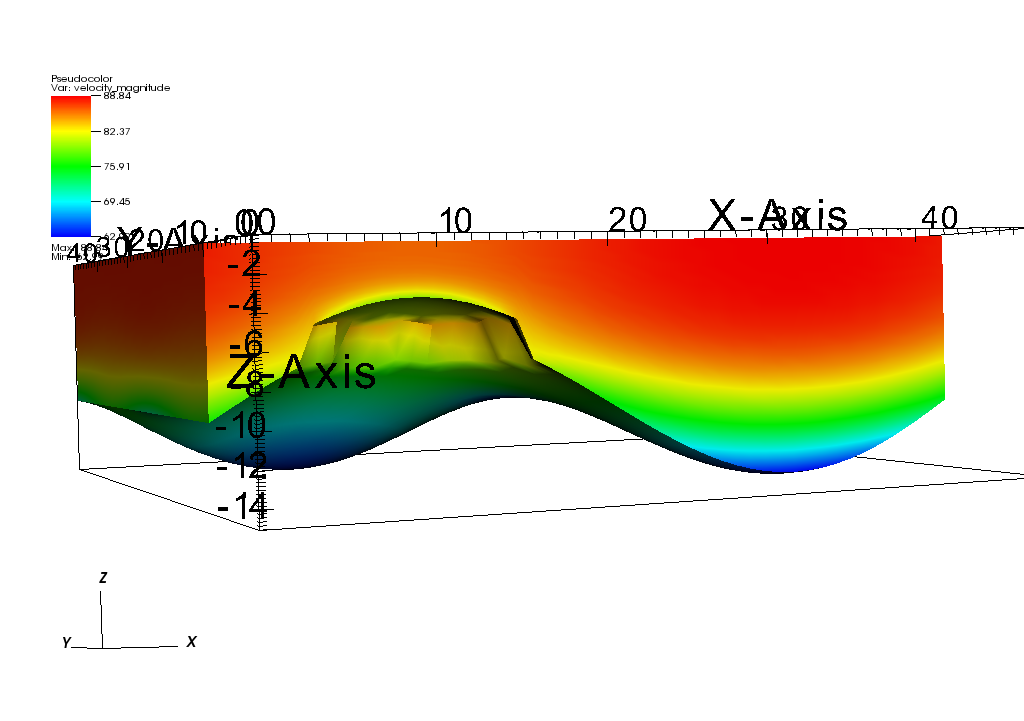
\includegraphics[width=\textwidth]{figures/THI/y-5km-m6p5l4-clip}
  \vspace{-3.5em}
  \begin{itemize}
  \item Bathymetry is essentially discontinuous on any grid
  \item Shallow ice approximation produces oscillatory solutions
  \item Nonlinear and linear solvers have major problems or fail
  \item Grid sequenced Newton-Krylov multigrid works \\
    as well as in the smooth case
  \end{itemize}
}

\begin{frame}
  \begin{figure}
    \includegraphics[width=\textwidth]{figures/THI/y-10km-m10p6l5-ew}
    \centering\caption{Grid sequenced Newton-Krylov convergence for test $Y$.
    The ``cliff'' has \SI{58}{\degree} angle in the red line ($12\times 125$ meter elements), \SI{73}{\degree} for the cyan line ($6\times 62$ meter elements).}\label{fig:testy}
  \end{figure}
\end{frame}
\begin{frame}
  \begin{figure}
    \includegraphics[width=\textwidth]{figures/THI/linear4}
    \centering\caption{Average number of Krylov iterations per nonlinear iteration.  Each nonlinear system was solved to a relative tolerance of $10^{-2}$.}\label{fig:linear}
  \end{figure}
\end{frame}
\begin{frame}
  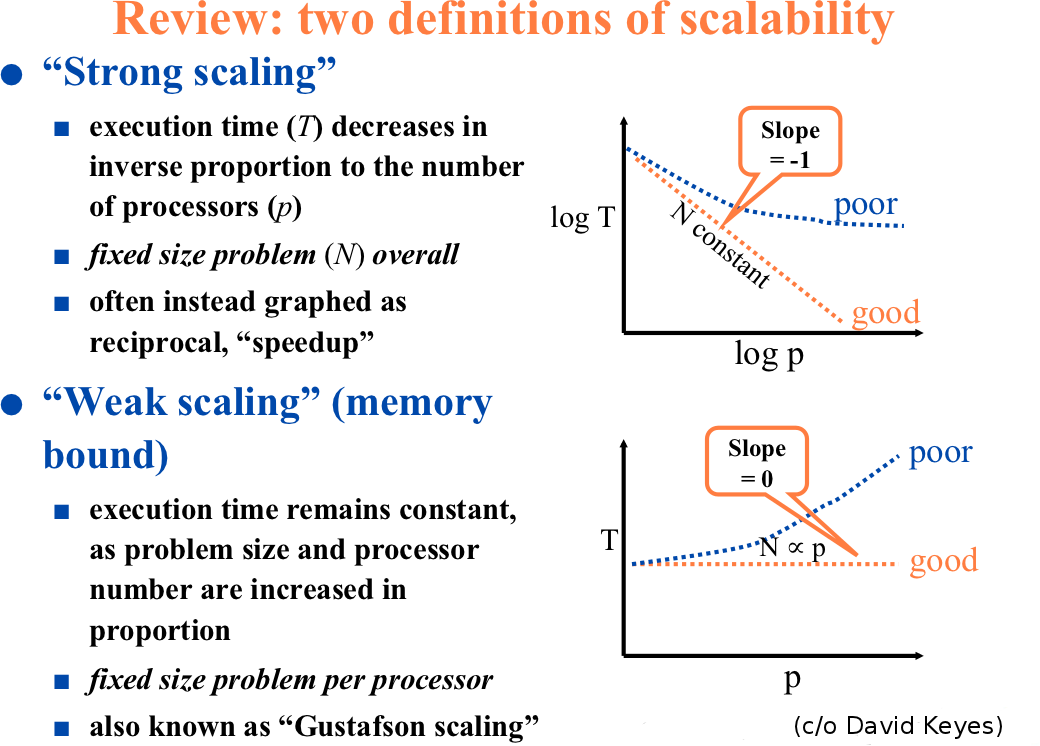
\includegraphics[width=\textwidth]{figures/KeyesStrongWeak} \\
  \uncover<2>{\large \alert{The easiest way to make software scalable is to make it sequentially inefficient. -- Gropp 1999}}
\end{frame}
\begin{frame}{Strong scaling on Blue Gene/P (Shaheen)}
\begin{figure}
  \includegraphics[width=\textwidth]{figures/THI/shaheen-strong}
  \centering\caption{Strong scaling on Shaheen for different size coarse levels problems and different coarse level solvers.
    The straight lines on the strong scaling plot have slope $-1$ which is optimal.}\label{fig:shaheen-strong}
\end{figure}
\end{frame}

\begin{frame}{Weak scaling on Blue Gene/P (Shaheen)}
  \begin{figure}
  \includegraphics[width=\textwidth]{figures/THI/shaheen-weak}
  \centering\caption{Weak scaling on Shaheen with a breakdown of time spent in different phases of the solution process.
    Times are for the full grid-sequenced problem, not just the finest level solve.}\label{fig:shaheen-weak}
\end{figure}
\end{frame}

\begin{frame}
  \begin{center}
    \alert{\huge One high-accuracy solve \\[0.2em]
      costs 30 times as much \\[0.5em]
      as a residual evaluation}
  \end{center}
  \begin{center}
    about 15 to reach truncation error

    \bigskip

    \uncover<2>{\alert{\Large 1000 times faster than methods currently in use} \\
      e.g. Lemieux, Price, Evans, Knoll, Salinger, Holland, Payne 2011 \\ (J. Computational Physics)}
    
    \bigskip

    {(Brown, Smith, Ahmadia 2011; submitted to SIAM J. Scientific Computing)}
  \end{center}
\end{frame}

\section{High throughput for high order finite elements}
\begin{frame}{What hardware is coming down the pike? (2018)}
  \begin{itemize}
  \item DOE Exascale program forecasts
    \begin{itemize}
    \item $10^6$ nodes, $10^3$ threads/node, $10$ GB/node, $10$ MB/thread
    \item 1--10 TF/node, \alert<2->{``balanced'' arithmetic intensity: 10--40 flops/byte}
    \item deep memory hierarchy, locality crucial, ``free'' flops
    \end{itemize}
  \item Arithmetic intensity: flops/byte
  \begin{itemize}
  \item sparse matrix kernels: 0.17--0.25
  \item matrix-free kernels: $\ge 5$
  \end{itemize}
\item Mitigation
  \begin{itemize}
  \item hierarchical methods with fewer/no global reductions
  \item reduce memory/bandwidth usage in exchange for more flops
    \begin{itemize}
    \item \alert<3>{higher order methods, recompute coefficients instead of storing}
    \end{itemize}
  \item ``communication avoiding'': apply operators multiple times while coefficients are in cache
    \begin{itemize}
    \item mathematics disagrees, sacrifice algorithmic scalability
    \end{itemize}
  \end{itemize}
\end{itemize}
\end{frame}

\begin{frame}[shrink=5]{Performance of assembled versus unassembled}
  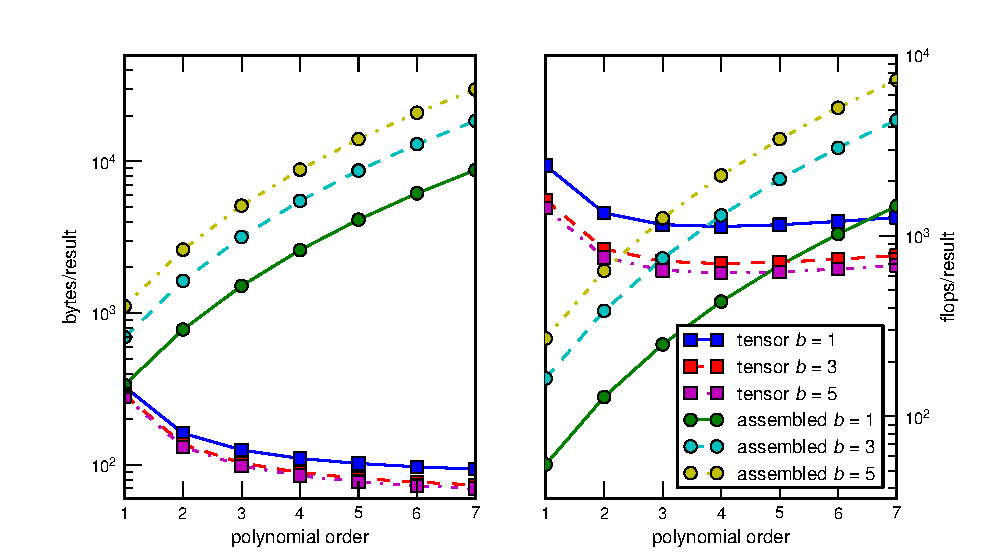
\includegraphics[width=\textwidth]{figures/TensorVsAssembly} \\
  \begin{itemize}
  \item High order Jacobian stored unassembled using coefficients at quadrature points, can use local AD
  \item Choose approximation order at run-time, independent for each field
  \item Precondition high order using assembled lowest order method
  \item Implementation $> 70\%$ of FPU peak, SpMV bandwidth wall $< 4\%$
  \end{itemize}
\end{frame}

\begin{frame}[shrink=5]{Representation of Jacobians, Automation}
  \begin{itemize}
  \item For unassembled representations, decomposition, and assembly
  \item Continuous weak form: find $u$
    \[ v^T F(u) \sim \int_\Omega v \cdot {\color{green!70!black} f_0(u,\nabla u)}
    + \nabla v \tcolon {\color{green!70!black} f_1(u,\nabla u)} = 0, \qquad \forall v \in \VV_0 \]
  \item Weak form of the Jacobian $J(u)$: find $w$
    \begin{gather*}
      v^T J(u) w \sim \int_\Omega \begin{bmatrix} v^T & \nabla v^T \end{bmatrix}
      {\color{blue} \begin{bmatrix} f_{0,0} & f_{0,1} \\ f_{1,0} & f_{1,1} \end{bmatrix}}
      \begin{bmatrix} w \\ \nabla w \end{bmatrix} \\
      {\color{blue} [f_{i,j}] = \begin{bmatrix} \dfrac{\partial f_0}{\partial u} & \dfrac{\partial f_0}{\partial \nabla u} \\[1em]
          \dfrac{\partial f_1}{\partial u} & \dfrac{\partial f_1}{\partial \nabla u} \end{bmatrix} (u,\nabla u) }
    \end{gather*}
  \item Terms in ${\color{blue} [f_{i,j}]}$ easy to compute symbolically, AD more scalable.
  \item Nonlinear terms ${\color{green!70!black}f_0,f_1}$ usually have the most expensive nonlinearities in the computation of scalars
    \begin{itemize}
    \item Equations of state, effective viscosity
    \item Compute gradient with reverse-mode, store at quadrature points.
    \item Perturb scalars, then use forward-mode to complete the Jacobian.
    \item Flip for action of the adjoint.
    \end{itemize}
  \end{itemize}
\end{frame}


% \begin{frame}{Verification and Validation}
  \begin{enumerate}
  \item Verification of code
    \begin{itemize}
    \item check that design order of the method is realized
    \item confirms that method is implemented correctly \\
      and the analysis of the method is correct
    \item manufactured solutions do not provide a proof, \\
      but are convincing as long as all terms are exercised
    \end{itemize}
  \item Verification of a computation
    \begin{itemize}
    \item a posteriori error estimates
    \item checking for mesh independence
    \item quantification of uncertainty from discretization and geometry/boundary conditions/materials
    \end{itemize}
  \item Validation of a computation
    \begin{itemize}
    \item needs high-quality laboratory/field measurements
    \item tests the quality of the continuum model
    \end{itemize}
  \end{enumerate}
  \begin{itemize}
  \item<2> \alert{Predictive modeling \textbf{only} after addressing all points above.}
  \end{itemize}
\end{frame}

% \begin{frame}[fragile,shrink=5]{Symbolic form of large-deformation elasticity}
  Find displacement vector $\uu$ such that:
  \begin{equation*}
    \int_\Omega \nabla \vv \tcolon \Pi = 0,\quad \forall \vv
  \end{equation*}
  where
  \begin{align*}
    F   & = I - \nabla \uu                &  & \text{Deformation gradient}  \\
    E   & = (F^T F - I)/2                 &  & \text{Green-Lagrange tensor} \\
    S   & = \lambda (\trace E) I + 2\mu E &  & \text{Second Piola-Kirchoff tensor} \\
\uncover<2>{\alert{S}   & \alert{ = \lambda (J^2 - I) C^{-1} + \mu (I - C^{-1})}} & & \uncover<2>{\text{Neo-Hookean material, } (C = F^T F)} \\
    \Pi & = F \cdot S                     &  & \text{First Piola-Kirchoff tensor}
  \end{align*}
  \vspace{-0.8em}
\begin{pythoncode}
  def weak_form(u, du, v, dv):
    I = eye(3)                      # Identity tensor
    F = I - du                      # Deformation gradient
    E = (F.T*F - I)/2               # Green-Lagrange tensor
    S = lmbda*E.trace()*I + 2*mu*E  # Second Piola-Kirchoff tensor
    Pi = F * S                      # First Piola-Kirchoff tensor
    return dv.dot(Pi)
\end{pythoncode}
\end{frame}

\begin{frame}[fragile]{Manufactured solution}
  \begin{itemize}
  \item Choose a solution $\uu_{\text{exact}}$ with rich derivatives
  \begin{pythoncode}
  def solution(x,y,z, a,b,c):
    return Matrix([cos(x) * exp(y) * z + sin(z),
                   sin(x) * tanh(y) + x * cosh(z),
                   exp(x) * sinh(y) + y * log(1+z**2)])
  \end{pythoncode}
  \item Apply strong-form nonlinear differential operator symbolically
    to define
    \[ f(x,y,z) = \nabla\cdot \Pi(\nabla \uu_{\text{exact}}) \]
  \item Solve finite element problem for $\uu_h$
    \begin{equation*}
      \int_\Omega \nabla \vv \tcolon \Pi(\nabla \uu_h) = \int v\cdot f(x,y,z),\quad \forall \vv
    \end{equation*}
  \item Compute norms of $\uu_h - \uu_{\text{exact}}$.
  \end{itemize}
\end{frame}

\begin{frame}{Manufactured solution}
  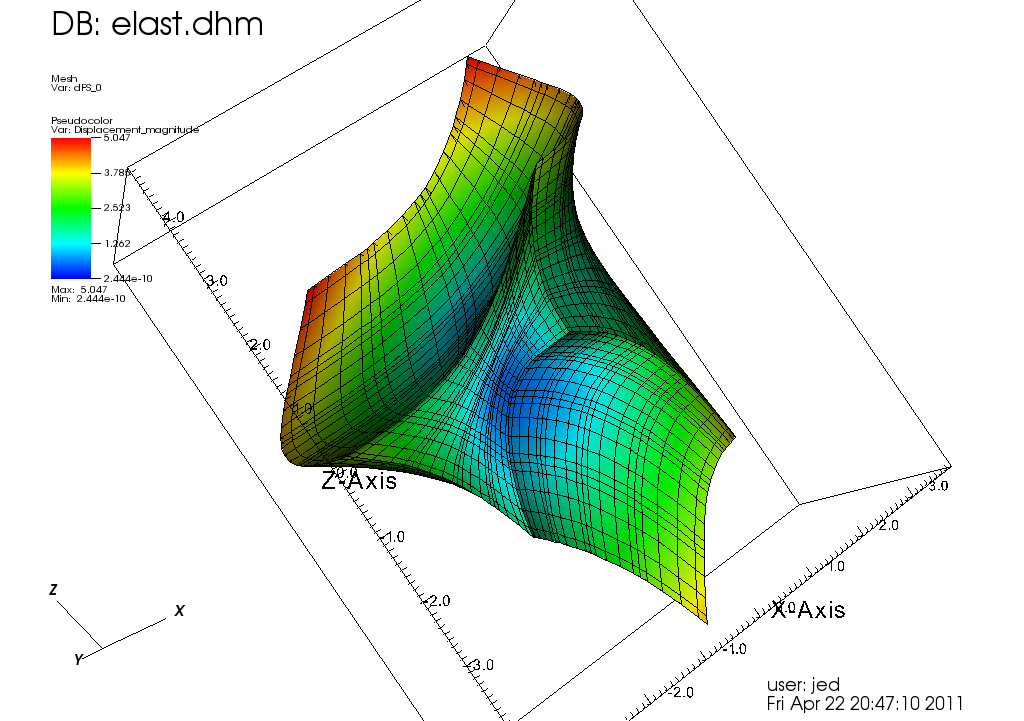
\includegraphics[width=\textwidth]{figures/elast-b4q5} \\
\end{frame}

\begin{frame}[shrink=30]{Convergence rates}
  \begin{tabular}{lrr rr rr rr rr}
    \toprule
    & & & \multicolumn{2}{c}{$\norm{\uu_h - \uu}_2$} & \multicolumn{2}{c}{$\norm{\uu_h - \uu}_\infty$}
    & \multicolumn{2}{c}{$\norm{\nabla\uu_h - \nabla\uu}_2$} & \multicolumn{2}{c}{$\norm{\nabla\uu_h - \nabla\uu}_\infty$} \\
    \cmidrule(r){4-5} \cmidrule(lr){6-7} \cmidrule(lr){8-9} \cmidrule(l){10-11}
    \multicolumn{2}{c}{Mesh} & \# Nodes & Error & \bigO & Error & \bigO & Error & \bigO & Error & \bigO \\
    \midrule % output below is generated with verif.py in this directory
$Q_1$ & $1^3$ & 8 & 1.79e+00 & --- & 6.50e-01 & --- & 3.70e+00 & --- & 1.08e+00 & --- \\
$Q_1$ & $2^3$ & 27 & 5.49e-01 & 1.71 & 3.40e-01 & 0.93 & 1.61e+00 & 1.20 & 6.92e-01 & 0.64 \\
$Q_1$ & $4^3$ & 125 & 1.53e-01 & 1.84 & 1.26e-01 & 1.43 & 8.01e-01 & 1.01 & 4.51e-01 & 0.62 \\
$Q_1$ & $8^3$ & 729 & 3.94e-02 & 1.96 & 3.73e-02 & 1.76 & 3.98e-01 & 1.01 & 2.81e-01 & 0.68 \\
$Q_1$ & $16^3$ & 4913 & 9.95e-03 & 1.99 & 1.01e-02 & 1.88 & 1.98e-01 & 1.01 & 1.57e-01 & 0.84 \\
$Q_1$ & $32^3$ & 35937 & 2.49e-03 & 2.00 & 2.61e-03 & 1.95 & 9.92e-02 & 1.00 & 8.32e-02 & 0.92\\
% \midrule
% $Q_2$ & $1^3$ & 27 & 2.44e-01 & --- & 1.82e-01 & --- & 9.48e-01 & --- & 4.60e-01 & --- \\
% $Q_2$ & $2^3$ & 125 & 3.71e-02 & 2.72 & 4.47e-02 & 2.03 & 2.86e-01 & 1.73 & 1.54e-01 & 1.58 \\
% $Q_2$ & $4^3$ & 729 & 4.48e-03 & 3.05 & 6.23e-03 & 2.84 & 6.94e-02 & 2.04 & 4.34e-02 & 1.83 \\
% $Q_2$ & $8^3$ & 4913 & 5.60e-04 & 3.00 & 9.31e-04 & 2.74 & 1.74e-02 & 2.00 & 1.29e-02 & 1.75 \\
% $Q_2$ & $16^3$ & 35937 & 7.01e-05 & 3.00 & 1.23e-04 & 2.92 & 4.34e-03 & 2.00 & 3.52e-03 & 1.87\\
\midrule
$Q_3$ & $1^3$ & 64 & 4.14e-02 & --- & 2.71e-02 & --- & 2.90e-01 & --- & 1.63e-01 & --- \\
$Q_3$ & $2^3$ & 343 & 2.06e-03 & 4.33 & 2.06e-03 & 3.72 & 2.39e-02 & 3.60 & 1.14e-02 & 3.84 \\
$Q_3$ & $4^3$ & 2197 & 1.81e-04 & 3.51 & 2.06e-04 & 3.32 & 4.23e-03 & 2.50 & 2.88e-03 & 1.98 \\
$Q_3$ & $8^3$ & 15625 & 1.22e-05 & 3.89 & 1.87e-05 & 3.46 & 5.79e-04 & 2.87 & 5.84e-04 & 2.30\\
\midrule
$Q_5$ & $1^3$ & 216 & 3.76e-03 & --- & 2.90e-03 & --- & 4.69e-02 & --- & 3.16e-02 & --- \\
$Q_5$ & $2^3$ & 1331 & 7.58e-05 & 5.63 & 5.92e-05 & 5.61 & 1.62e-03 & 4.86 & 1.05e-03 & 4.91 \\
$Q_5$ & $4^3$ & 9261 & 7.33e-07 & 6.69 & 6.61e-07 & 6.48 & 2.59e-05 & 5.97 & 1.76e-05 & 5.90\\
% \midrule
% $Q_7$ & $1^3$ & 512 & 4.46e-04 & --- & 3.59e-04 & --- & 8.15e-03 & --- & 5.83e-03 & --- \\
% $Q_7$ & $2^3$ & 3375 & 2.95e-06 & 7.24 & 2.95e-06 & 6.93 & 8.21e-05 & 6.63 & 6.05e-05 & 6.59 \\
% $Q_7$ & $4^3$ & 24389 & 7.65e-09 & 8.59 & 1.07e-08 & 8.11 & 4.09e-07 & 7.65 & 3.95e-07 & 7.26\\
\midrule
$Q_9$ & $1^3$ & 1000 & 5.81e-05 & --- & 5.04e-05 & --- & 1.42e-03 & --- & 1.05e-03 & --- \\
$Q_9$ & $2^3$ & 6859 & 6.27e-08 & 9.86 & 7.59e-08 & 9.38 & 1.63e-06 & 9.77 & 1.60e-06 & 9.36 \\
\bottomrule
  \end{tabular}
\end{frame}


\section{Algebraic coupling algorithms and interfaces}
\begin{frame}{The Great Solver Schism: Monolithic or Split?}
  \begin{columns}
    \begin{column}{0.5\textwidth}
      \begin{block}{Monolithic}
        \begin{itemize}
        \item Direct solvers
        \item Coupled Schwarz
        \item Coupled Neumann-Neumann \\
          (need unassembled matrices)
        \item Coupled multigrid
        \item[X] Need to understand local spectral and compatibility properties of the coupled system
        \end{itemize}
      \end{block}
    \end{column}
    \begin{column}{0.5\textwidth}
      \begin{block}{Split}
        \begin{itemize}
        \item Physics-split Schwarz \\
          (based on relaxation)
        \item Physics-split Schur \\
          (based on factorization)
          \begin{itemize}
          \item  approximate commutators \\
            SIMPLE, PCD, LSC
          \item segregated smoothers
          \item Augmented Lagrangian
          \item ``parabolization'' for stiff waves
          \end{itemize}
        \item[X] Need to understand global coupling strengths
        \end{itemize}
      \end{block}
    \end{column}
  \end{columns}
  \begin{itemize}
  \item Preferred data structures depend on which method is used.
  \item Interplay with geometric multigrid.
  \end{itemize}
\end{frame}

\begin{frame}{Multi-physics coupling in PETSc}
  \begin{columns}
    \begin{column}{0.5\textwidth}
      \tikzstyle{cloud} = [draw, ellipse,fill=red!20, node distance=3cm, minimum height=2em]
      \tikzstyle{block} = [rectangle, draw, fill=blue!20, text width=5em, text centered, rounded corners, minimum height=2em]
      \begin{tikzpicture}
        \node [cloud] (momentum) {Momentum};
        \node [cloud, right of=momentum] (pressure) {Pressure};
        \node<2-> [block, opacity=0.5, fit=(momentum)(pressure), text opacity=0.8] (stokes) {Stokes};
        \node<3-> [cloud, below=2em of momentum] (energy) {Energy};
        \node<3-> [cloud, below=2em of pressure] (geometry) {Geometry};
        \node<4-> [block, opacity=0.4, fit=(stokes)(momentum)(pressure)(energy)(geometry), text opacity=0.8, text height=4em] (ice) {Ice};
        \node<5-> [block, below=2em of ice, minimum width=16em] (bl) {{Boundary \nolinebreak Layer}};
        \node<5-> [block, below=2em of bl, minimum width=16em] (ocean) {Ocean};
        % ]
      \end{tikzpicture}
    \end{column}
    \begin{column}{0.5\textwidth}
      \begin{itemize}
      \item package each ``physics'' independently
      \item solve single-physics and coupled problems
      \item semi-implicit and fully implicit
      \item reuse residual and Jacobian evaluation unmodified
      \item direct solvers, fieldsplit inside multigrid, multigrid inside fieldsplit without recompilation
      \item use the best possible matrix format for each physics \\ (e.g. symmetric block size 3)
      \item matrix-free anywhere
      \item multiple levels of nesting
      \end{itemize}
    \end{column}
  \end{columns}
\end{frame}

\begin{frame}
  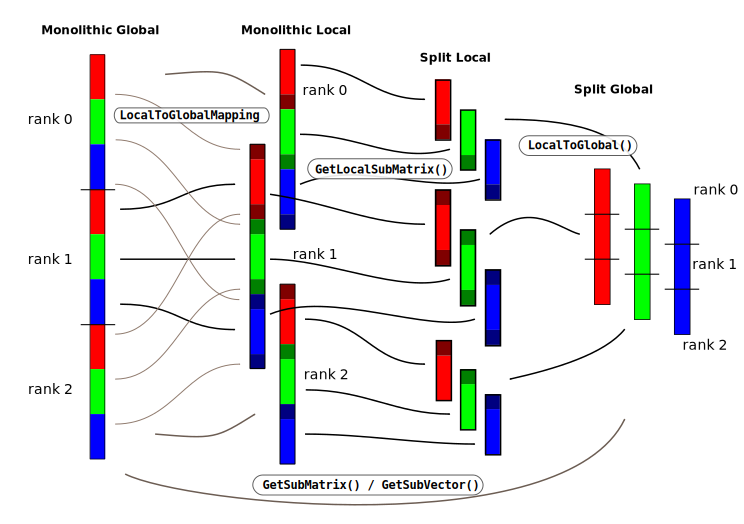
\includegraphics[width=\textwidth]{figures/PETSc/LocalSpaces} \\[-.5em]
  Work in Split Local space, matrix data structures reside in any space.
\end{frame}

\begin{frame}
  \alert{\texttt{MatGetLocalSubMatrix(Mat A,IS rows,IS cols,Mat *B);}}
  \begin{itemize}
  \item Primarily for assembly
    \begin{itemize}
    \item \texttt{B} is not guaranteed to implement \texttt{MatMult}
    \item The communicator for \texttt{B} is not specified, \\
      only safe to use non-collective ops (unless you check)
    \end{itemize}
  \item \texttt{IS} represents an index set, includes a block size and communicator
  \item \texttt{MatSetValuesBlockedLocal()} is implemented
  \item MatNest returns nested submatrix, no-copy
  \item No-copy for Neumann-Neumann formats \\ (unassembled across procs, e.g. BDDC, FETI-DP)
  \item Most other matrices return a lightweight proxy \texttt{Mat}
    \begin{itemize}
    \item \texttt{COMM\_SELF}
    \item Values not copied, does not implement \texttt{MatMult}
    \item Translates indices to the language of the parent matrix
    \item Multiple levels of nesting are flattened
    \end{itemize}
  \end{itemize}
\end{frame}


\section{Conservative polythermal ice flow}
\newcommand\smallterm[1]{{\color{gray} #1}}
\begin{frame}{Conservative two-phase formulation}
  Find momentum density $\rho\uu$, pressure $p$, and total energy density $E$:
  \begin{gather*}
    (\rho\uu)_t + \div (\smallterm{\rho\uu\otimes\uu} - \eta D\uu_i + p\bm 1) - \rho \bm g = 0 \\
    \rho_t + \div \rho\uu = 0 \\
    E_t + \div \big((E+p)\uu - k_T\nabla T - k_\omega\nabla\omega \big) - \eta D\uu_i\tcolon D\uu_i - \smallterm{\rho\uu\cdot\bm g} = 0
  \end{gather*}
\begin{itemize}
\item Solve for density $\rho$, ice velocity $\uu_i$, temperature $T$, and melt fraction $\omega$ using constitutive relations.
  \begin{itemize}
  \item Simplified constitutive relations can be solved explicitly.
  \item Temperature, moisture, and strain-rate dependent rheology $\eta$.
  \item High order FEM, typically $Q_3$ momentum \& energy, SUPG (yuck).
  \end{itemize}
\item DAEs solved implicitly after semidiscretizing in space.
\item Newton solver converges quadratically.
\item Thermocoupled steady state in one nonlinear solve
  \begin{itemize}
  \item no time stepping needed, total cost similar to 3 semi-implicit steps
  \item useful for inverse problems and stability analysis
  \end{itemize}
\item (Somewhat) robust preconditioning using nested field-split
\end{itemize}
\end{frame}

\begin{frame}{Block on inclined plate, nominal $\Reynolds = 0.24$, $\Peclet = 120$}
  \begin{columns}
    \begin{column}{0.5\textwidth}
      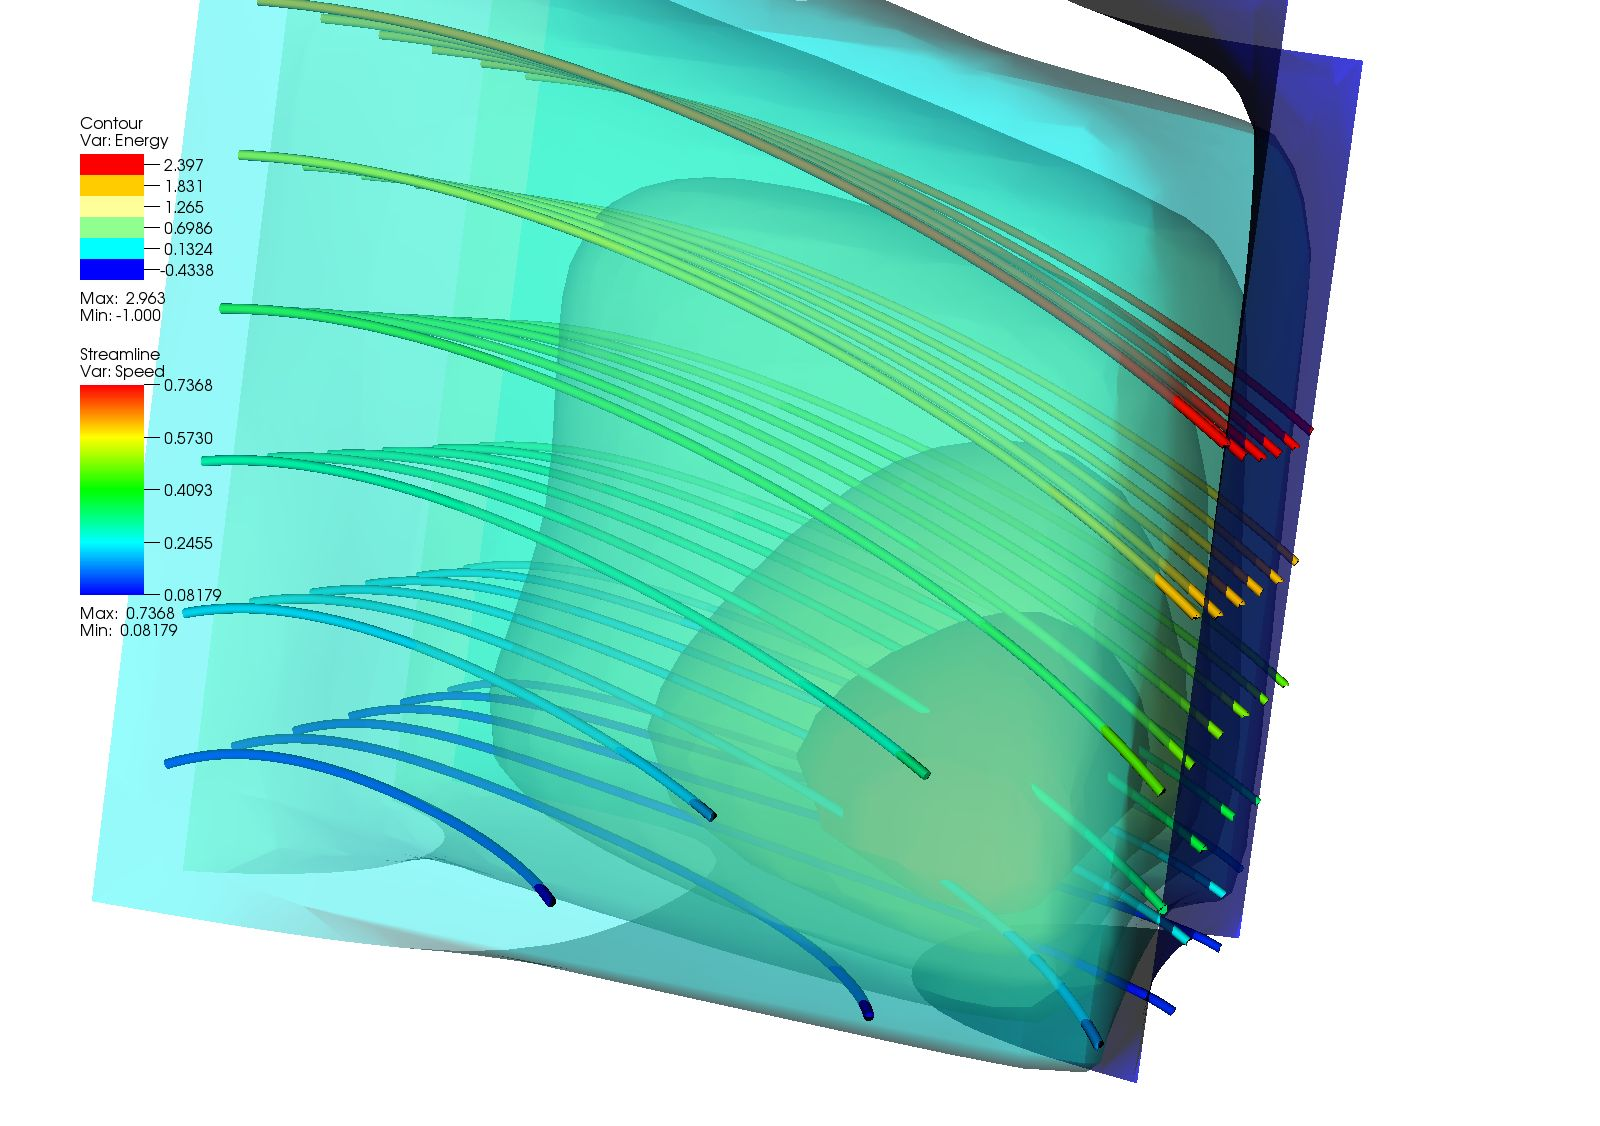
\includegraphics[width=1.3\textwidth]{figures/VHTNondimEnergy} \\
      Contours of Energy, melt fraction up to 15\%, density ratio 2.
    \end{column}
    \begin{column}{0.5\textwidth}
      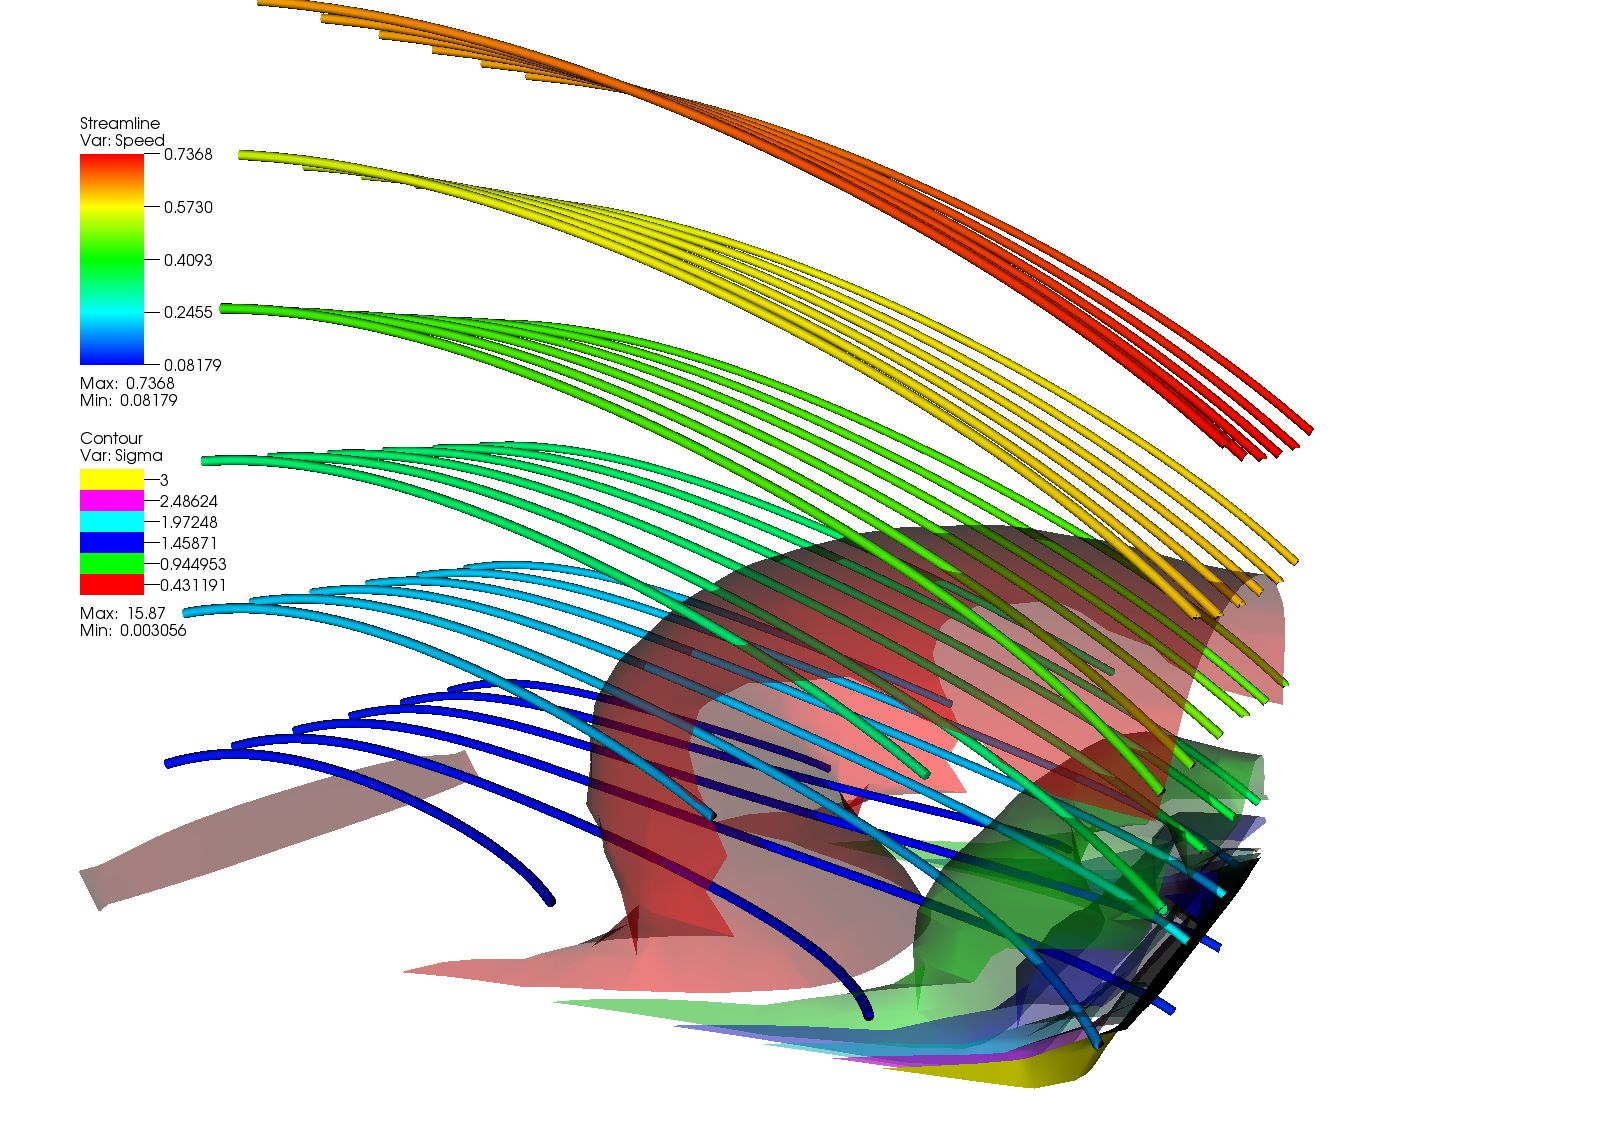
\includegraphics[width=1.3\textwidth]{figures/VHTNondimSigma} \\
      Contours of viscous heat production, $1/r$ singularity at corners.
    \end{column}
  \end{columns}
\end{frame}

\begin{frame}{Relative effect of the blocks}
  \begin{equation*}\label{eq:vhtblock}
    J =
    \begin{pmatrix}
      J_{uu} & J_{up} & J_{uE} \\
      J_{pu} & 0 & 0 \\
      J_{Eu} & J_{Ep} & J_{EE}
    \end{pmatrix} .
  \end{equation*}
  \begin{itemize}
  \item[$J_{uu}$] Viscous/momentum terms, nearly symmetric, variable coefficionts, anisotropy from Newton.
  \item[$J_{up}$] Weak pressure gradient, viscosity dependence on pressure (small), gravitational contribution (pressure-induced density variation).
    Large, nearly balanced by gravitational forcing.
  \item[$J_{uE}$] Viscous dependence on energy, very nonlinear, not very large.
  \item[$J_{pu}$] Divergence (mass conservation), nearly equal to $J_{up}^T$.
  \item[$J_{Eu}$] Sensitivity of energy on momentum, mostly advective transport.
    Large in boundary layers with large thermal/moisture gradients.
  \item[$J_{Ep}$] Thermal/moisture diffusion due to pressure-melting, $\uu \cdot \nabla$.
  \item[$J_{EE}$] Advection-diffusion for energy, very nonlinear at small regularization.
    Advection-dominated except in boundary layers and stagnant ice, often balanced in vertical.
  \end{itemize}
\end{frame}

\begin{frame}{How much nesting?}
  \begin{columns}
    \begin{column}{0.5\textwidth}
      \begin{equation*}
        P_1 =
        \begin{pmatrix}
          J_{uu} & J_{up} & J_{uE} \\
          0 & B_{pp} & 0 \\
          0 & 0 & J_{EE} \\
        \end{pmatrix}
      \end{equation*}
      \begin{itemize}
      \item $B_{pp}$ is a mass matrix in the pressure space weighted by inverse of kinematic viscosity.
      \item Elman, Mihajlovi\'c, Wathen, JCP 2011 for non-dimensional isoviscous Boussinesq.
      \item Works well for non-dimensional problems on the cube, not for realistic parameters.
      \end{itemize}
    \end{column}
    \begin{column}{0.5\textwidth}
      \begin{equation*}
        P =
        \begin{bmatrix}
          \begin{pmatrix}
            J_{uu} & J_{up} \\
            J_{pu} & 0
          \end{pmatrix} & \\
          \begin{pmatrix}
            J_{Eu} & J_{Ep}
          \end{pmatrix}
          & J_{EE}
        \end{bmatrix}
      \end{equation*}
      \begin{itemize}
      \item Inexact inner solve using upper-triangular with $B_{pp}$ for Schur.
      \item Another level of nesting.
      \item GCR tolerant of inexact inner solves.
      \item Outer converges in 1 or 2 iterations.
      \end{itemize}
    \end{column}
  \end{columns}
  \begin{itemize}
  \item Low-order preconditioning full-accuracy unassembled high order operator.
  \item Build these on command line with PETSc \cverb|PCFieldSplit|.
  \end{itemize}
\end{frame}


%\begin{frame}[shrink=5]{Everything is better as a smoother (sometimes)}
  \begin{block}{Block preconditioners work alright, but\ldots}
    \begin{itemize}
    \item nested iteration requires more dot products
    \item more iterations: coarse levels don't ``see'' each other
    \item finer grained kernels: lower arithmetic intensity, even more limited by memory bandwidth
    \end{itemize}
  \end{block}
  \begin{block}{Coupled multigrid}
    \begin{itemize}
    \item need compatible coarsening
      \begin{itemize}
      \item can do algebraically (Adams 2004) but would need to assemble
      \end{itemize}
    \item stability issues for lowest order $Q_1-P_0^{\text{disc}}$
      \begin{itemize}
      \item Rannacher-Turek looks great, but no discrete Korn's inequality
      \end{itemize}
    \item coupled ``Vanka'' smoothers difficult to implement with high performance, especially for FEM
    \item block preconditioners as smoothers reuse software better
    \item one level by reducing order for the coarse space, more levels need non-nested geometric MG or go all-algebraic and pay for matrix assembly and setup
    \end{itemize}
  \end{block}
\end{frame}

\begin{frame}
  \centering
  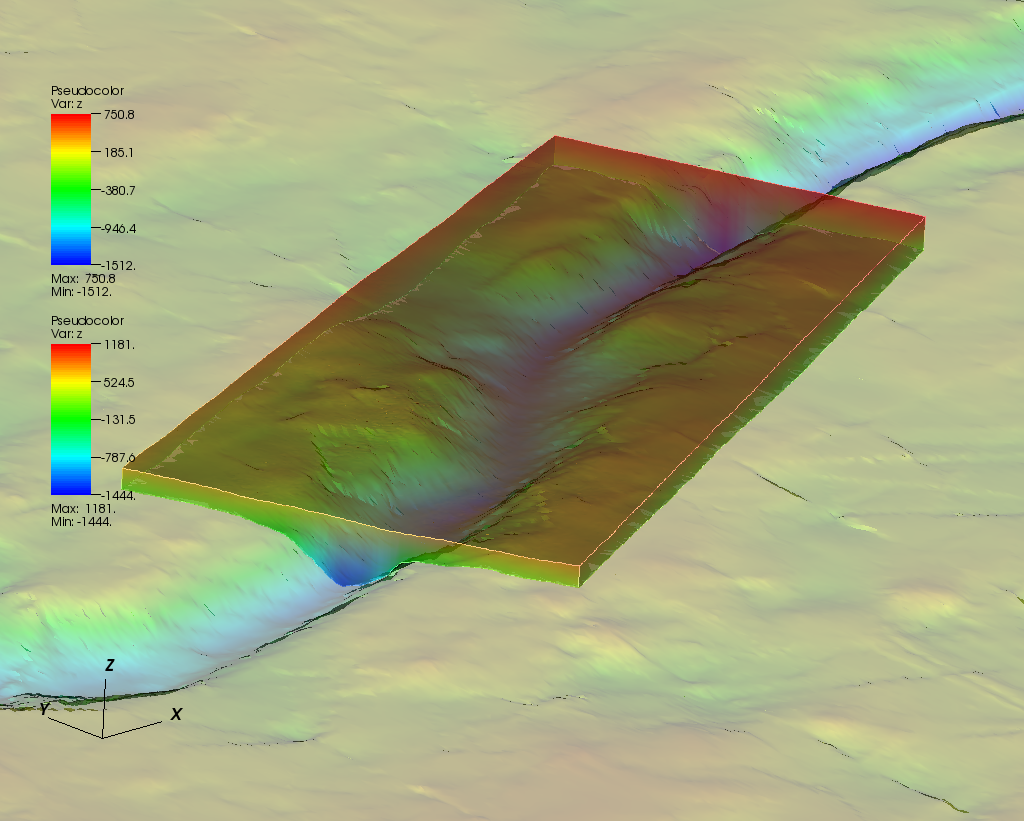
\includegraphics[width=\textwidth]{figures/jakotransparent}
\end{frame}

\begin{frame}
  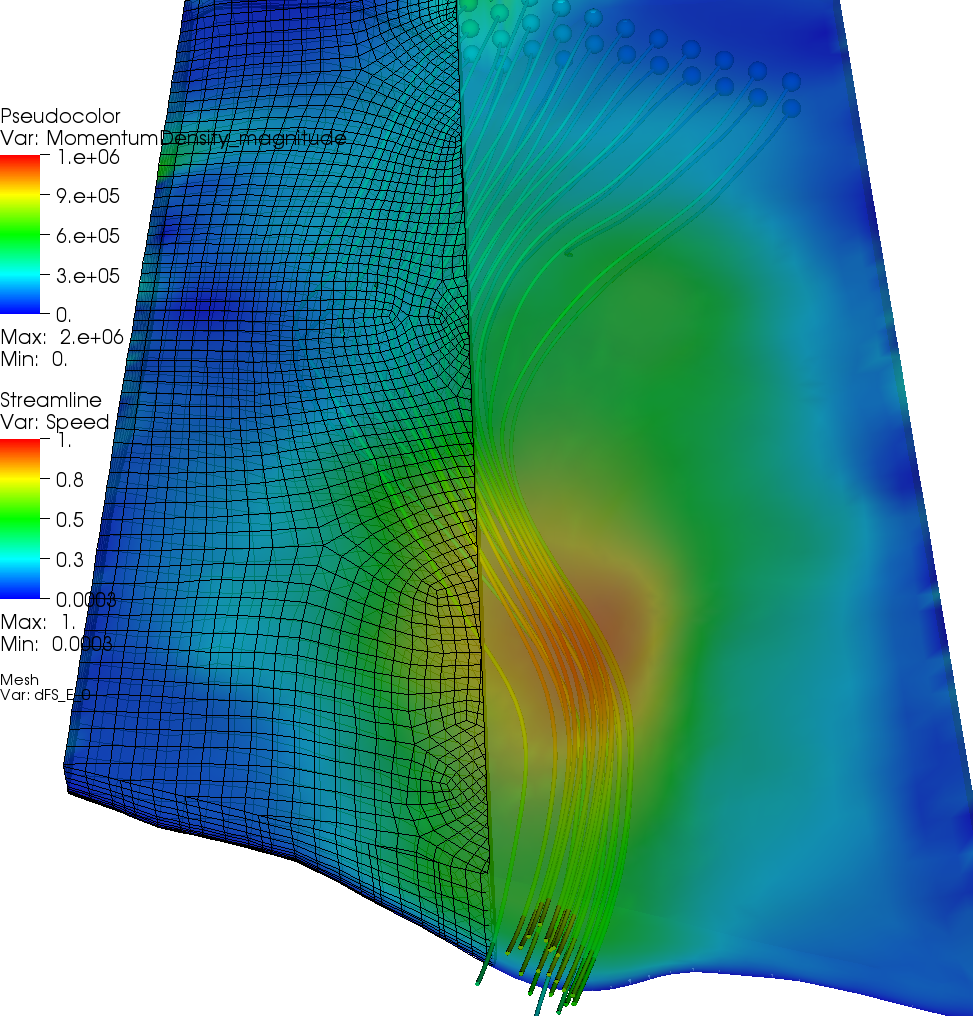
\includegraphics[width=\textwidth]{figures/VHT/TopViewStreamline}
\end{frame}

\begin{frame}
  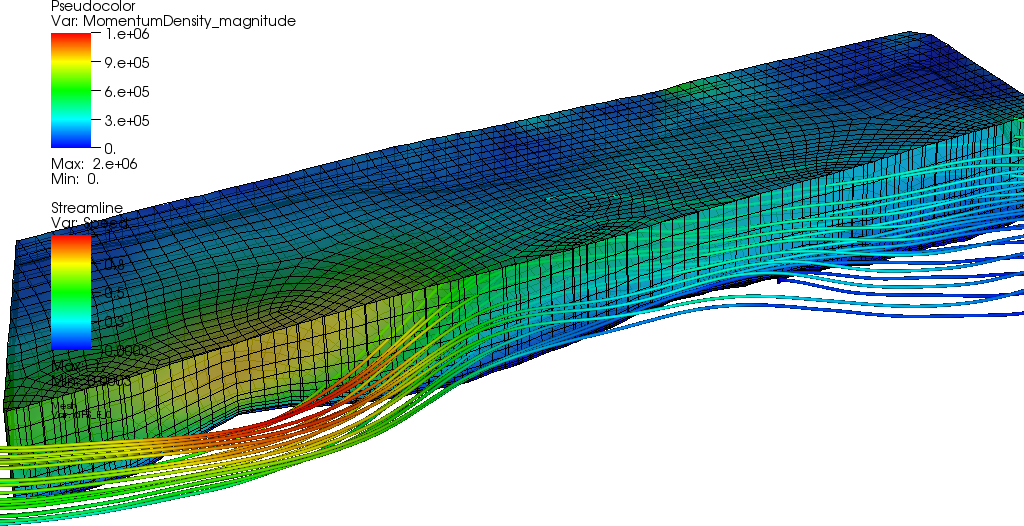
\includegraphics[width=0.9\textwidth]{figures/VHT/JakoSideMomentum} \\
  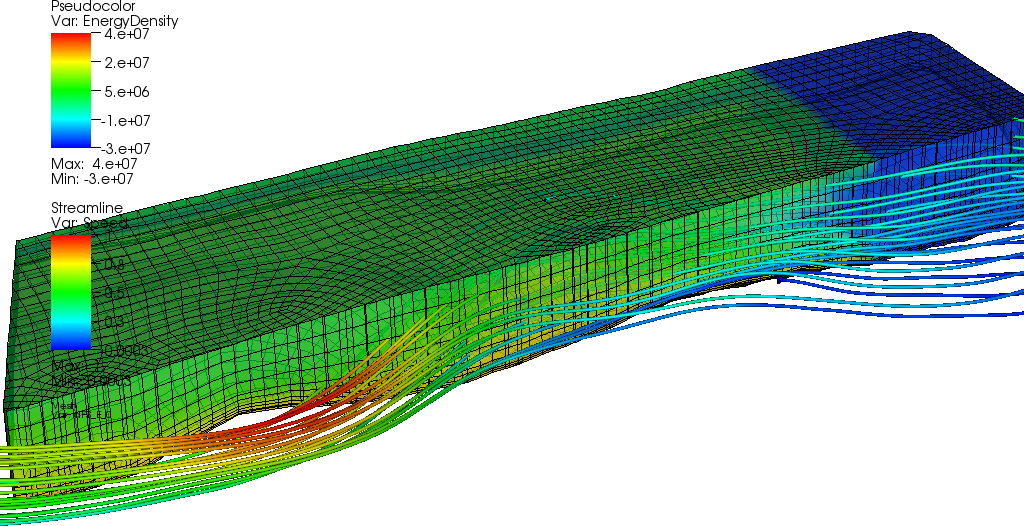
\includegraphics[width=0.9\textwidth]{figures/VHT/JakoSideEnergy}
\end{frame}


\begin{frame}{Summary}
  \begin{itemize}
  \item textbook multigrid efficiency for hydrostatic ice
  \item dual-order $h$ and $p$-version finite element library
    \begin{itemize}
    \item alleviate memory bandwidth bottleneck by factor of 50
    \item run-time choice of order, compatibility for mixed spaces
    \item $>70\%$ of FPU peak for core library kernels
    \item geometric model is available to physics/solvers
    \item automation of code verification
    \end{itemize}
  \item bridging the Great Solver Schism
    \begin{itemize}
    \item commuting multilevel methods with field-splitting
    \item data structure independence for assembly
    \item decouple software packaging from available solution algorithms
    \end{itemize}
  \item technical requirements for robust discretizations of ice flow
  \item 3D implicit polythermal ice flow
    \begin{itemize}
    \item new conservative formulation
    \item quadratically convergent steady-state solver
    \item run in Jakobshavn geometry
    \end{itemize}
  \end{itemize}
\end{frame}

\begin{frame}{Outlook}
  \begin{itemize}
  \item Need better transport algorithm: discontinuous Galerkin
  \item Many flavors of contact: large-deformation, self, frictional, thermal
  \item Unstructured geometric multigrid/full-space DD
  \item Non-interactive remeshing after topology change/large deformation
  \item Move from symbolics to AD for manufactured solutions/codegen
  \item IMEX methods now implemented $G(t,x,\dot x) = F(t,x)$
  \item General/nonsymmetric pivoting for full-space optimization
  \item Uncertainty quantification for semi-smooth systems
  \item Multi-parameter continuation for stability analysis
  \end{itemize}
\end{frame}

\end{document}
